\documentclass{article}
\usepackage[utf8]{inputenc}
\usepackage{graphicx}
\usepackage{amsmath}

\title{Sight Distance}
\author{Ayush Pandey}
\date{July 2019}

\begin{document}

\maketitle

\section{Issues}
    The term \emph{"sight distance"} used below is the distance from the car to the farthest point on the road that falls on the line of sight of the driver. This \textbf{needs to be replaced with a more appropriate term.} Similarly, the term \emph{"object distance"} is used to depict the farthes distance upto which an object is visible to the river, this too \textbf{needs to be rectified.}

\section{The Problem}
    Given a vertical curve with initial gradient $g_{1}$, a transition curve of length $l$ and a final gradient $-g_{2}$, we find the farthest distance where an object will be visible to a driver.\\
    The only known parameters in the problem are $g_{1}$, $g_{2}$, $l$, height of the car $h_{c}$ and the height of the object $h_{o}$.
    
\section{The Road's Equation}
    We assume that the initial approach is linear with gradient $g_{1}$, the transition curve is a quadratic curve and the final approach is also linear with the gradient $-g_{2}$. Let the intersection (at A) of the initial approach  and the transition curve be the origin. The transition and the final section intersect at some point B.The setup is shown in figure \ref{fig:RoadEqn}.
    
    \begin{figure}[h]
        \centering
        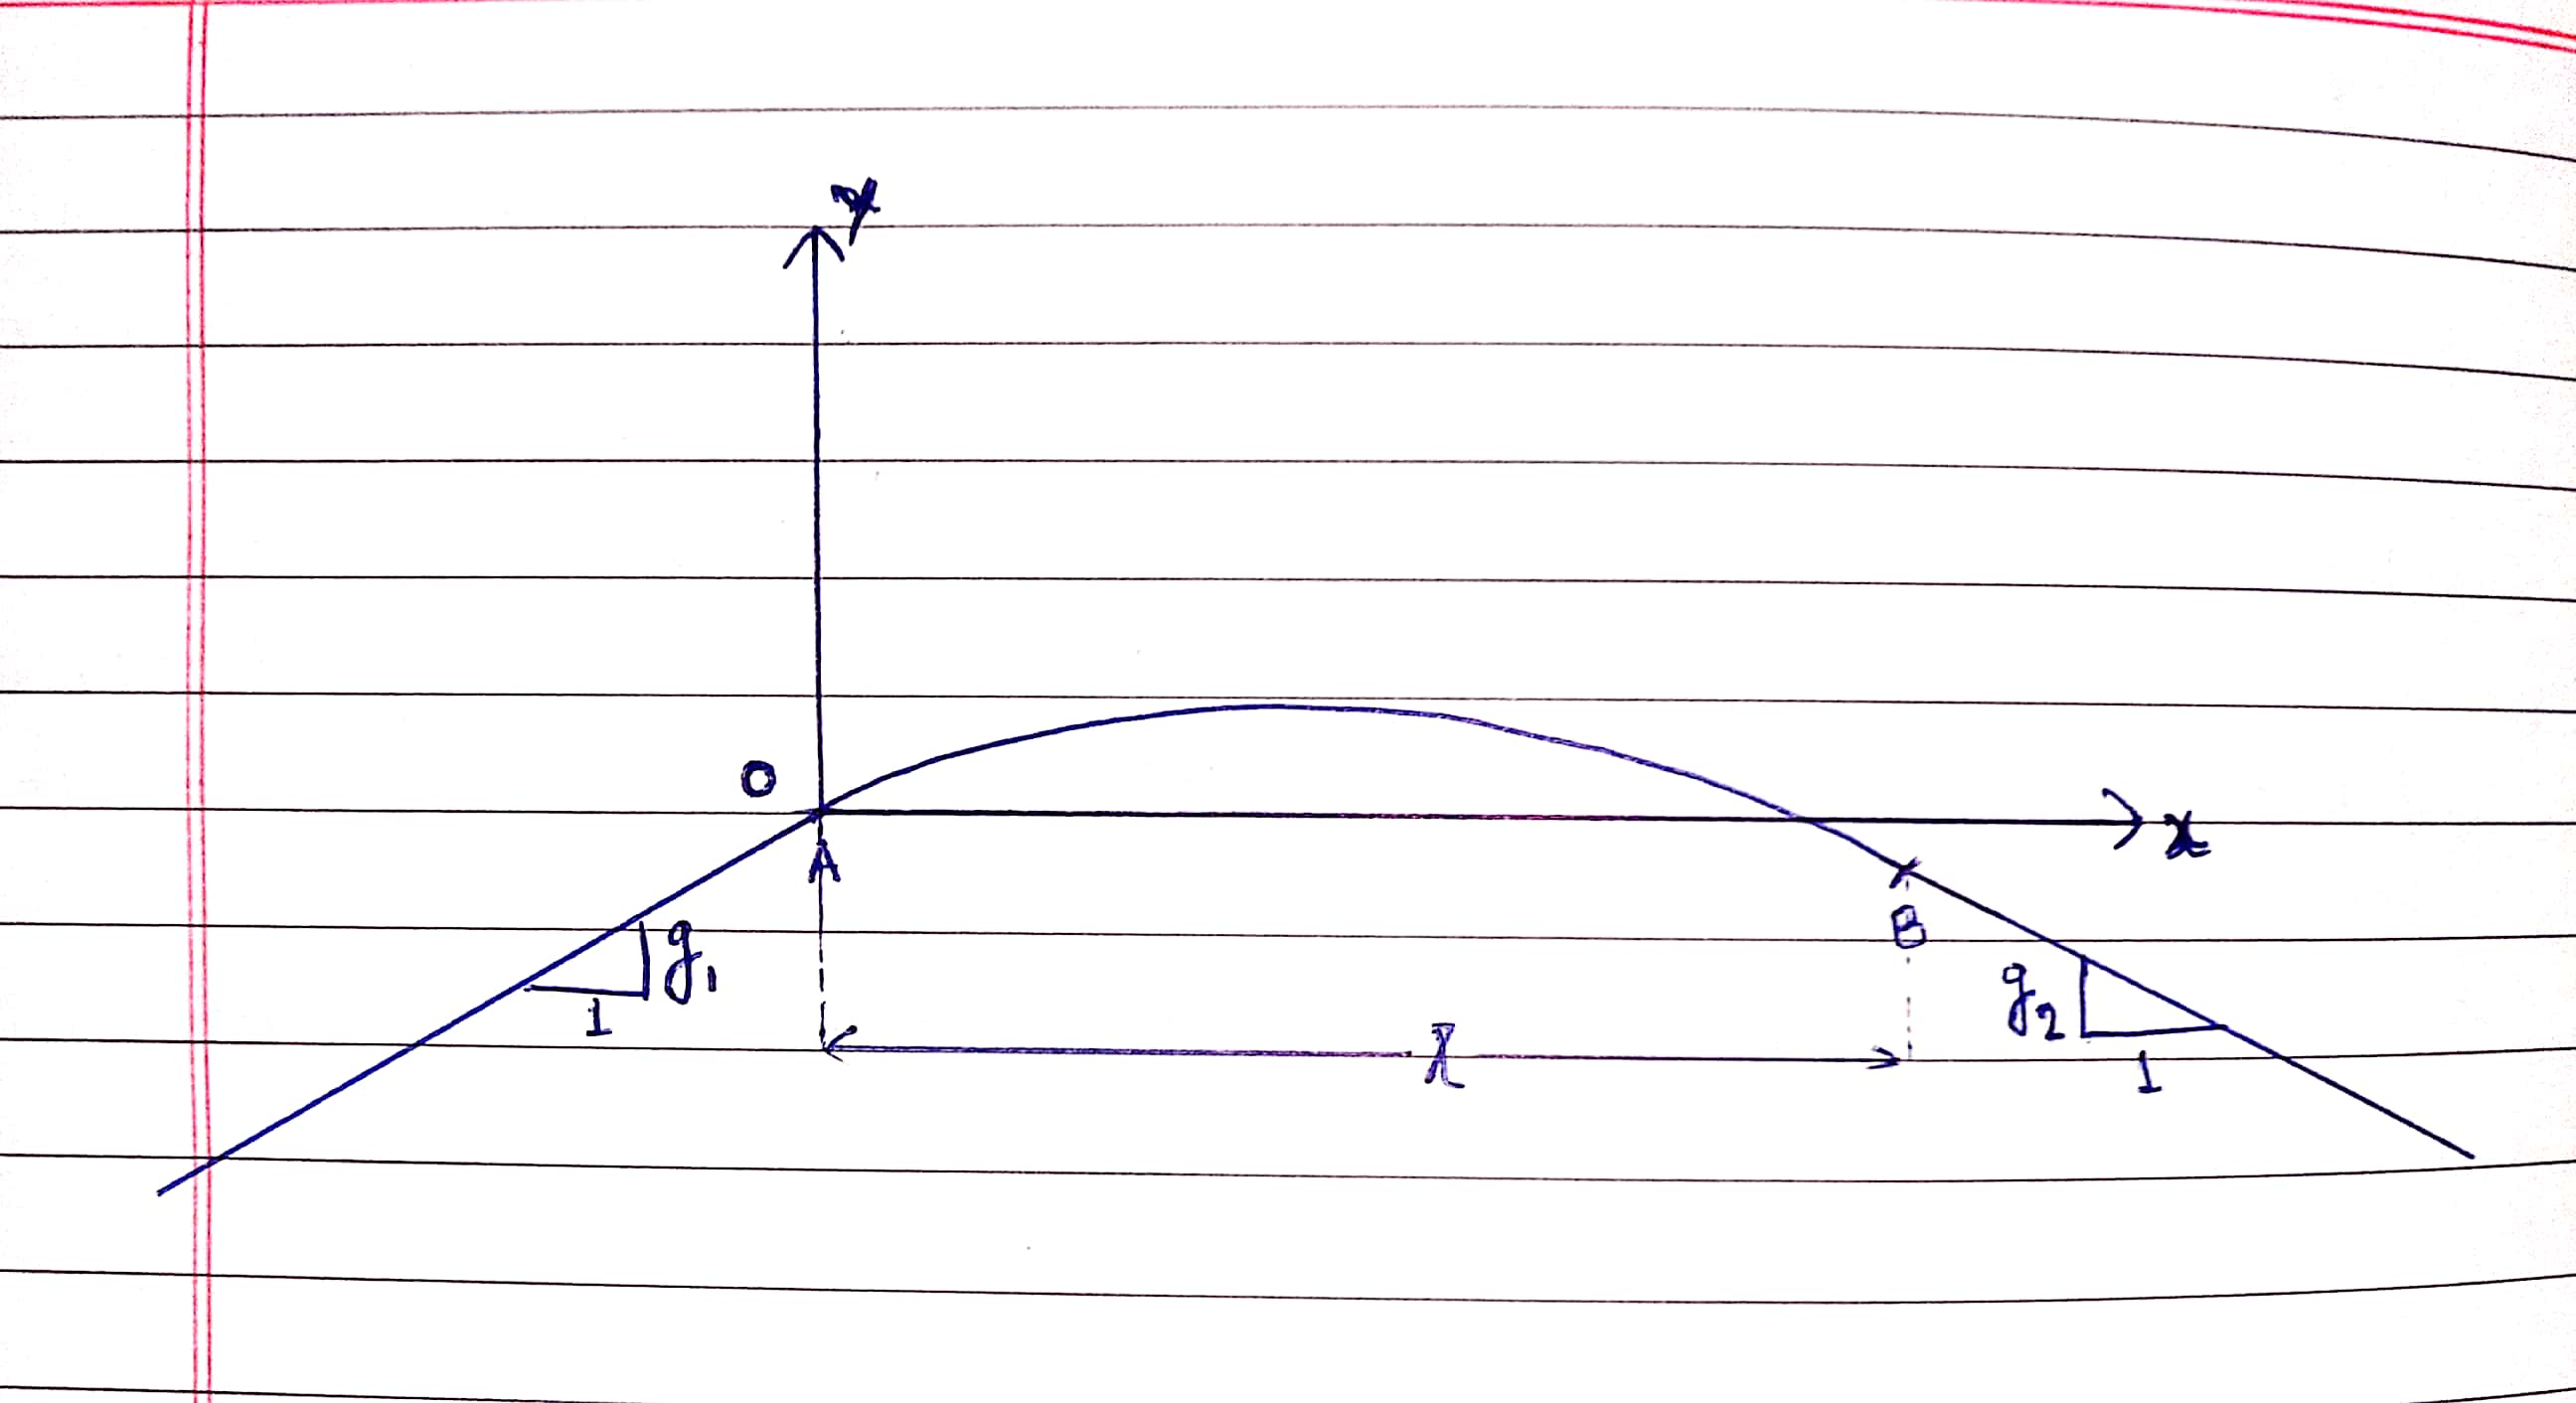
\includegraphics[width = \textwidth]{RoadEqn.jpg}
        \caption{Side view of road geometry}
        \label{fig:RoadEqn}
    \end{figure}
    
    Let us depict the elevation of the road with regards to $x$ using road as $y_{r}$. Since the road is made of three different sections, we need three equation to depict the road as a piecewise function. The piece before the origin, i.e., $x < 0$ is a simple line passing through the origin with gradient $g_{1}$, the transition curve is quadratic with slope $g_{1}$ at $x = 0$ and $-g_{2}$ at $x = l$, the section is a line with slope $-g_{2}$. This can be written as equation \ref{eq:1}.
    
    \begin{equation} \label{eq:1}
        y_{r}(x) = 
            \begin{cases}
                g_{1}x &\quad\forall \hspace{0.2cm} x < 0\\
                ax^{2} + bx + c &\quad\forall \hspace{0.2cm} 0 \leq x < l\\
                -g_{2}x + k &\quad\forall \hspace{0.2cm} l \leq x\\
            \end{cases}    
    \end{equation}
    
    The above equation should be continuous and differentiable. The three piecewise function are themselves differentiable so we check only for $x = 0$ and $x = l$. This gives us four conditions, $y_{r}(0-) = y_{r}(0+)$; $y_{r}'(0) = g_{1}$; $y_{r}'(l) = -g_{2}$ and $y_{r}(l-) = y_{r}(l+)$.\\
    
    Using the above conditions, we get $y_{r}$ in equation \ref{eq:2}.

    \begin{equation} \label{eq:2}
        y_{r}(x) = 
            \begin{cases}
                g_{1}x &\quad\forall \hspace{0.2cm} x < 0\\
                -\frac{g_{1} + g_{2}}{2l}x^{2} + g_{1}x &\quad\forall \hspace{0.2cm} 0 \leq x < l\\
                \frac{g_{1} + g_{2}}{2}l - g_{2}x &\quad\forall \hspace{0.2cm} l \leq x\\
            \end{cases}    
    \end{equation}
    
    The slope of the road can be depicted as $y_{r}'$ given in equation \ref{eq:3}
    
    \begin{equation} \label{eq:3}
        y_{r}'(x) = 
            \begin{cases}
                g_{1} &\quad\forall \hspace{0.2cm} x < 0\\
                -\frac{g_{1} + g_{2}}{l}x + g_{1} &\quad\forall \hspace{0.2cm} 0 \leq x < l\\
                -g_{2} &\quad\forall \hspace{0.2cm} l \leq x\\
            \end{cases}    
    \end{equation}
    
\section{Equation of Tangent}
    The line of sight of the driver is tangent to the road and in this case, usually to the transition curve. We can compute the equation of the tangent hitting the curve at point $(x_{m}, y_{r}(x_{m}))$. The equation is of the form $mx + c$ with $m = y_{r}'(x_{m})$ and $c$ can be computed by substituting the point of contact $(x_{m}, y_{r}(x_{m}))$ into the equation.
    
    \begin{equation*}
        y_{r}(x_{m}) = mx_{m} + c
    \end{equation*}
    
    \begin{equation*}
        \implies y_{r}(x_{m}) = y_{r}'(x_{m})x_{m} + c
    \end{equation*}
    
    \begin{equation*}
        \implies c = y_{r}(x_{m}) - y_{r}'(x_{m})x_{m}
    \end{equation*}
    
    Hence the equation of the line is of the form given in equation \ref{eq:4}.
    
    \begin{equation} \label{eq:4}
        \left \{ x, y_{r}'(x_{m})(x - x_{m}) + y_{r}(x_{m}) \right \}
    \end{equation}
    
\section{Finding the point of contact of tangent $x_{m}$ given the position of car $x_{c}$}
    We need to find the sight distance for the while moving, the position of the car depends on its speed and acceleration and the sight distance depends on its position. If we can thus find a general formulation for the sight distance given the position of the car to obtain the sight distance for each instant based on the car's speed and time passed.\\
    Let's say that the car is at $x_{c}$ and the eye of the driver is at a height $h_{c}$ above the ground. The position of the eye of the driver, $y_{c}$ hence is,
    
    \begin{equation*}
        y_{c}(x) = y_{r}(x) + h_{c}
    \end{equation*}
    
    The line of sight passes through the eye of the driver and is tangent to the road. Since it is tangent to the road, it would be in the form of equation \ref{eq:4}. $(x_{c}, y_{c}(x_{c}))$ falls on this line. Hence we can write
    
    \begin{equation*}
        y_{c}(x_{c}) = y_{r}'(x_{m})(x_{c} - x_{m}) + y_{r}(x_{m})
    \end{equation*}
    
    and we can hence write
    
    \begin{equation} \label{eq:5}
        y_{r}'(x_{m})(x_{c} - x_{m}) + y_{r}(x_{m}) - y_{r}(x_{c}) - h_{c} = 0
    \end{equation}
    
    We can solve equation \ref{eq:5}, a quadratic in $x_{m}$, for $x_{m}$ as we know $x_{c}$. The equation of the line of sight can then be calculated using the two points $(x_{c}, y_{c}(x_{c}))$ and $(x_{m}, y_{r}(x_{m}))$.
    
\section{Calculating Object Distance}
    We can calculate the object distance, the farthest distance which the driver can see an object of height $h_{o}$. Let  us say that the driver can see the object as far as $x_{o}$, then the point $y_{r}(x_{o}) + h_{o}$ falls on the line of sight calculated using $(x_{c}, y_{c}(x_{c}))$ and $(x_{m}, y_{r}(x_{m}))$. Substituting $(x_{o}, y_{r}(x_{o}) + h_{o})$ in the line of sight and solving for $x_{o}$ gives us the object distance.
    
\section{Solving Equation \ref{eq:5}}
    \begin{equation*}
        y_{r}'(x_{m})(x_{c} - x_{m}) + y_{r}(x_{m}) - y_{r}(x_{c}) - h_{c} = 0
    \end{equation*}
    
    \begin{equation*}
        \implies y_{r}'(x_{m})x_{c} - y_{r}'(x_{m})x_{m} + y_{r}(x_{m}) - y_{r}(x_{c}) - h_{c} = 0
    \end{equation*}
    
    \begin{equation*}
        \implies \left ( g_{1} - \frac{g_{1} + g_{2}}{l}x_{m} \right ) x_{c} - \left ( g_{1} - \frac{g_{1} + g_{2}}{l}x_{m} \right ) x_{m} + \left ( g_{1}x_{m} - \frac{g_{1} + g_{2}}{2l}x_{m}^{2} \right ) + \left ( -y_{r}(x_{c}) - h_{c} \right ) = 0
    \end{equation*}
    
    \begin{equation*}
        \implies x_{m}^{2}\left ( \frac{g_{1} + g_{2}}{l} - \frac{g_{1} + g_{2}}{2l} \right ) + x_{m}\left ( -\frac{g_{1} + g_{2}}{l}x_{c} - g_{1} + g_{1} \right ) + \left ( g_{1}x_{c} - y_{r}(x_{c}) - h_{c} \right ) = 0
    \end{equation*}
    
    \begin{equation} \label{eq:6}
        \implies x_{m}^{2}\left ( \frac{g_{1} + g_{2}}{2l} \right ) - x_{m}\left ( \frac{g_{1} + g_{2}}{l}x_{c} \right ) + \left ( g_{1}x_{c} - y_{r}(x_{c}) - h_{c} \right ) = 0
    \end{equation}
    
    Equation \ref{eq:6} is based on the assumption that the line of sight is tangent to a point of a transition curve and not on the approach or final curve. Plugging in the values, one can solve for $x_{m}$
    
\end{document}
